\chapter{Analisis Masalah Pengumpulan Data Pada \textit{Spreadsheet}}

Pada bab ini diuraikan analisis persoalan pengumpulan data pada \textit{spreadsheet} yang telah diuraikan pada Bab I. Hasil dari bab ini digunakan untuk merancang aplikasi yang akan diimplementasikan seperti yang dijelaskan pada Bab IV.

\section{Permasalahan Pengumpulan Data Pada \textit{Spreadsheet}} \label{AspekAplikasi}
Pada Subbab \ref{RumusanMasalah} telah dijelaskan bahwa terdapat tiga permasalahan yang muncul didalam pengumpulan data menggunakan media \textit{spreadsheet} yakni:
\begin{enumerate}
	\item Kolaborasi \\
	Didalam pembuatan suatu \textit{spreadsheet}, kadang dibutuhkan banyak pihak untuk dapat melengkapi seluruh data yang dibutuhkan. Hal ini membuat pengembangan dan pengumpulan data membutuhkan kontribusi banyak orang \citep{Panko1998}. Untuk itu dibutuhkan fitur kolaborasi pada aplikasi \textit{spreadsheet} agar banyak pihak dapat melakukan pengumpulan data dan pengeditan secara bersamaan.
	\item Validasi \\
	Data yang dikumpulkan pada suatu \textit{spreadsheet}, sangat rentan akan kesalahan. Bahkan pada \textit{spreadsheet} yang dibuat dengan sangat hati-hati, masih dapat ditemui sekitar 1 persen atau lebih kesalahan pada formula yang dibuat \citep{Panko1998}. Sehingga dibutuhkan mekanisme tambahan pada saat pengumpulan data untuk melakukan validasi terhadap masukan.
	\item Penyimpanan Data \\
	Setelah data dikumpulkan, permasalahan selanjutnya yang muncul adalah penyimpanan data tersebut. Data biasanya akan tetap tersimpan dalam bentuk berkas \textit{spreadsheet}, namun bentuk ini sulit untuk digunakan oleh aplikasi lain. Bentuk yang biasanya digunakan oleh aplikasi lain untuk dapat mengambil dan menyimpan data adalah bentuk relasional. Sehingga dibutuhkan mekanisme penyimpanan data ke dalam bentuk relasional agar data dapat dengan mudah digunakan pada aplikasi lain.
\end{enumerate}

Ketiga permasalahan tersebut yang dijadikan dasar pengembangan aplikasi pada Tugas Akhir ini dan akan dibahas pada subbab-subbab berikutnya. 

% Pada Subbab \ref{KesalahanPenggunaan} dijelaskan bahwa terdapat dua jenis kesalahan yang dapat terjadi pada penggunaan \textit{spreadsheet} yakni kesalahan kualitatif dan kesalahan kuantitatif. Kesalahan kualitatif merupakan kesalahan penggunaan \textit{spreadsheet} yang berhubungan dengan kualitas dan prosedur penggunaan. Contoh kesalahan kualitatif yang sering terjadi adalah penggunaan \textit{spreadsheet} sebagai basis data. Kesalahan kuantitatif merupakan kesalahan yang menyebabkan keluaran menjadi salah. Contoh kesalahan kuantitatif yang sering terjadi adalah kesalahan masukan yang tidak divalidasi.

% Pencegahan untuk kesalahan-kesalahan ini dapat dilihat pada Subbab \ref{PenangananKesalahan}. Salah satu caranya adalah pembuatan \textit{preliminary design} terhadap \textit{spreadsheet} yang dibuat. Hal ini dapat dilakukan dengan cara pengembangan aplikasi pengumpulan data berbentuk \textit{spreadsheet} yang menangani kolaborasi, validasi, dan penyimpanan. Dengan aplikasi ini diharapkan dapat menangani kesalahan kualitatif seperti yang dijelaskan pada contoh sebelumnya yakni penggunaan \textit{spreadsheet} sebagai basis data dengan cara menghubungkan \textit{spreadsheet} ke basis data yang sesungguhnya secara langsung. Serta menangani kesalahan kuantitatif dengan cara melakukan validasi masukan.

% Aplikasi \textit{spreadsheet} yang baik harus dapat diakses dan digunakan secara kolaboratif yang dapat dilakukan dengan membuat aplikasi \textit{spreadsheet} tersebut berbasis \textit{web}. Aspek-aspek aplikasi \textit{web} yang perlu diperhatikan dalam membangun aplikasi \textit{spreadsheet} adalah:
% \begin{enumerate}
% 	\item \textit{Response time}\\
% 	Membangun aplikasi berbasis \textit{web} menggunakan HTTP sebagai protokol komunikasi dan tentunya didalam komunikasi tersebut membutuhkan waktu untuk mengirimkan \textit{request} dari klien. Jika waktu yang dibutuhkan untuk melakukan respon lambat, akan sulit terjadi kolaborasi dan memperbesar kemungkinan terjadinya \textit{race condition} pada masukan pengguna. Sehingga diperlukan waktu respon yang cepat untuk dapat menangani banyak \textit{request} dalam satu waktu dan dalam waktu yang singkat.

% 	\item Akses yang konkuren\\
% 	Aplikasi berbasis \textit{web} yang akan dibuat harus dapat diakses secara konkuren yakni diakses bersama-sama oleh banyak klien dalam satu waktu. Pengaksesan secara konkuren dapat berdampak pada terpanggilnya banyak \textit{query} dalam satu waktu. Oleh karena itu aplikasi yang dibuat harus dapat menjalankan secara konkuren setiap \textit{request} yang masuk.

% 	\item Akses basis data\\
% 	Akses terhadap basis data dibutuhkan sebagai media penyimpanan yang persisten dan konsisten. Oleh karena itu, akses terhadap basis data diperlukan untuk kemudahan penyimpanan dan pengambilan data serta mengatasi permasahalan ketidaksamaan \textit{versioning} diantara suatu \textit{file spreadsheet}.

% \end{enumerate}

% Keempat aspek pada aplikasi berbasis \textit{web} tersebut akan menjadi aspek utama yang dikembangkan didalam pembuatan aplikasi \textit{spreadsheet} berbasis aplikasi \textit{web}.

% Berdasarkan pada Subbab \ref{KesalahanPenggunaan}, terdapat dua jenis tipe kesalahan \citep{Panko1998} yang bisa terjadi pada penggunaan \textit{spreadsheet} yakni:
% \begin{enumerate}
% 	\item Kesalahan Kualitatif

% 	Kesalahan kualitatif merupakan kesalahan yang berhubungan dengan kualitas yang dipengaruhi oleh prosedur pembuatan dan rancangan pada \textit{spreadsheet} tersebut. Contoh kesalahan kualitatif yang sering terjadi adalah penggunan \textit{spreadsheet} sebagai media penyimpanan atau basis data. Hal ini tidak sesuai dengan kegunaan utama dari \textit{spreadsheet} sebagai media kalkulasi dan perhitungan statistik.

% 	\item Kesalahan Kuantitatif

% 	Kesalahan kuantitatif merupakan kesalahan yang menyebabkan hasil perhitungan menjadi salah atau tidak valid. Contoh kesalahan jenis ini yang sering terjadi adalah kesalahan mekanikal dimana pengguna salah memasukan data yang tidak sesuai dengan konstrain yang ada. Hal ini dapat diatasi dengan adanya validasi sebelum data diterima. 
% \end{enumerate}

% Dari kedua tipe tersebut, pada Tugas Akhir ini akan lebih ditekankan kepada kesalahan kuantitatif yang bertipe kesalahan mekanikal dengan memanfaatkan teknik validasi pada masukan. 

% Dengan menggunakan aplikasi ini, terdapat perubahan alur penggunaan \textit{spreadsheet}. Gambar dibawah ini merupakan alur penggunaan aplikasi \textit{spreadsheet} biasa pada Gambar \ref{GambarWorkflowBiasa} dan aplikasi \textit{spreadsheet} yang dibangun pada Tugas Akhir ini pada Gambar \ref{GambarWorkflow}. 

% 	\begin{figure}[htb]
% 	    \centering
% 	    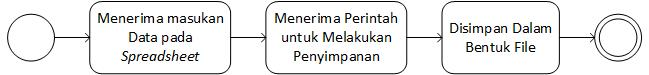
\includegraphics[width=0.7\textwidth]{resources/chapter-3-workflow-biasa.jpg}
% 	    \caption{Alur Kerja Aplikasi \textit{Spreadsheet} Biasa}
% 		\label{GambarWorkflowBiasa}
% 	\end{figure}

% 	\begin{figure}[htb]
% 	    \centering
% 	    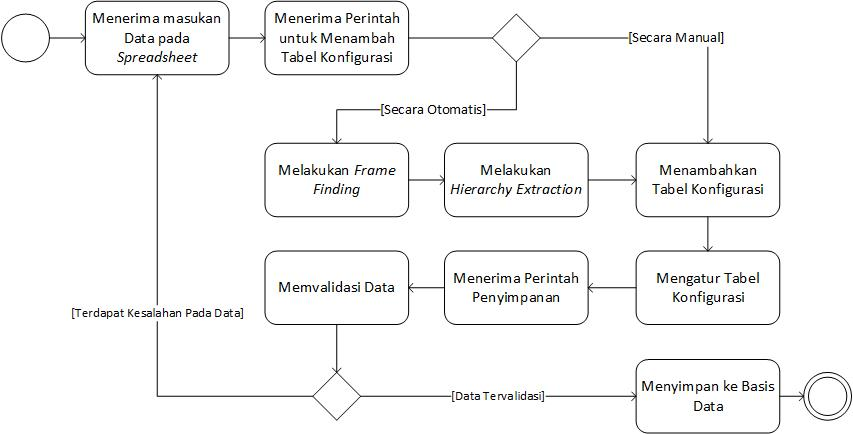
\includegraphics[width=1\textwidth]{resources/chapter-3-workflow.jpg}
% 	    \caption{Alur Kerja Aplikasi \textit{Spreadsheet} yang Akan Dibuat}
% 		\label{GambarWorkflow}
% 	\end{figure}

% Dapat dilihat bahwa terdapat proses tambahan yang dilakukan pada aplikasi yang akan dibuat. Proses tersebut terdiri dari pencarian bagian label dan data serta proses validasi. Hasil dari identifikasi label dan data akan dijadikan \textit{tuple} relasional yang disimpan dalam bentuk basis data.

\section{Analisis Rancangan Aplikasi \textit{Spreadsheet}}
Dari permasalahan yang telah didefinisikan pada subbab \ref{AspekAplikasi}, dapat ditentukan beberapa hal yang harus dianalisis dalam merancang aplikasi \textit{spreadsheet} ini, diantaranya adalah:
\begin{enumerate}
	\item Penentuan aplikasi \textit{spreadsheet} yang akan dikembangkan dan ditambahkan fiturnya. Aplikasi harus memiliki fitur kolaborasi sehingga banyak pengguna dapat mengakses suatu \textit{spreadsheet} secara bersamaan.
	\item Penanganan konflik yang terjadi pada saat kolaborasi.
	\item Jenis \textit{spreadsheet} yang menjadi fokus utama untuk dapat ditangani oleh aplikasi.
	\item Pemilihan metode interaksi aplikasi \textit{spreadsheet} dimana pengguna dapat membentuk struktur tempat pengguna lain memasukkan masukan. Contohnya dalam bentuk tabel atau formulir. Pengguna juga melengkapi domain dan batasan data yang dimasukkan.
	\item Setelah pengguna selesai merancang struktur masukan, diperlukan penentuan bagian label dan data yang berkaitan dengan label tersebut. Bagian label dan data akan dijadikan menjadi bentuk relasional yang dapat disimpan dalam basis data.
	\item Setelah label dan data ditentukan, tabel harus direpresentasikan dalam bentuk relasional sehingga dapat dimasukkan ke dalam basis data.
	\item Setelah data dikumpulkan, data perlu divalidasi dan dicek kesesuaiannya sesuai dengan batasan yang diberikan sehingga memenuhi domain yang ditentukan pada basis data.
	\item Setelah proses validasi terpenuhi, diperlukan cara penyimpanan data sesuai dengan relasi \textit{tuple} yang telah ditentukan.
	\item Interaksi antar \textit{spreadsheet} yang ingin memasukkan data pada suatu tabel yang sama perlu ditangani dan ditentukan aturannya.
\end{enumerate}
Pada subbab-subbab selanjutnya, akan dibahas analisis untuk kelima poin diatas yang selanjutnya akan dijadikan dasar rancangan fitur yang akan dibuat pada aplikasi \textit{spreadsheet}.

\section{Analisis Perbandingan Aplikasi \textit{Spreadsheet} yang Dikembangkan}
Dari studi yang telah dilaksanakan pada subbab \ref{TeknologiSpreadsheet}, aplikasi \textit{spreadsheet} dapat dibagi berdasarkan konektivitasnya yakni \textit{offline spreadsheet} dan \textit{online spreadsheet} dan dapat juga dibagi lagi berdasarkan keterbukaan dari \textit{source code} yakni \textit{open source} dan \textit{closed source}. Pada Tabel \ref{AnalisisAplikasiDasar} dijabarkan parameter yang mendasari pemilihan aplikasi yang akan dikembangkan.

\begin{small}
\begin{longtable}{ | p{3cm} | p{4cm} | p{4cm} | }
    \caption{Perbandingan Aplikasi \textit{Spreadsheet}}
    \label{AnalisisAplikasiDasar}\\ \hline
    \centering\bfseries{Parameter} & \centering\bfseries{Offline Application} & \centering\bfseries{Web/Online Application} \tabularnewline \hline
    \endfirsthead
    \hline
    \centering\bfseries{Parameter} & \centering\bfseries{Offline Application} & \centering\bfseries{Web/Online Application} \tabularnewline \hline
    \endhead
    Aksesibilitas & Dibutuhkan instalasi aplikasi / plugin yang bersangkutan. & Dapat menggunakan web browser yang tersedia. \\ \hline
    Kolaborasi & Tidak tersedia secara online dan kolaboratif secara \textit{default}. & Secara \textit{default}, dapat diakses konkuren dan kolaboratif. \\ \hline
    Fitur & Sudah banyak jenis formula yang didukung. & Tidak semua formula yang ada didukung. \\ \hline
\end{longtable}
\end{small}

Dari perbandingan diatas, diambil solusi dengan menggunakan aplikasi \textit{spreadsheet} berbasis web yang dapat diakses secara konkuren dan memiliki \textit{portability} yang lebih baik. Selain itu, untuk dapat mengembangkan fitur aplikasi dengan lebih baik, akan dipilih aplikasi yang berbentuk \textit{open source}. Alasan lain dipilihnya \textit{open source} adalah aplikasi berbasis \textit{open source} dapat dipasang pada \textit{platform} yang diinginkan oleh pengguna. Pengguna atau perusahaan yang menggunakan aplikasi dapat membangun infrastrukturnya sendiri sehingga dapat mengatur privasi dan performa aplikasi sesuai dengan keinginan pengguna. Sehingga dipilih aplikasi yang memiliki tipe \textit{online spreadsheet} dan \textit{open source} yaitu EtherCalc. Fitur kolaborasi yang dibutuhkan akan ditangani oleh aplikasi EtherCalc ini dan bukan merupakan bagian dari fitur yang akan dikembangkan.

\section{Analisis Penanganan Konflik saat Kolaborasi}
Penanganan konflik telah ditangani oleh EtherCalc menggunakan mekanisme \textit{conflict resolution} yang berasal dari SocialCalc. Mekanisme penanganan konflik menggunakan fitur \textit{undo}/\textit{redo} yang telah ada. Berdasarkan website resmi dari EtherCalc, langkah-langkah penanganan konflik yang terjadi adalah sebagai berikut,

\begin{enumerate}
	\item Ketika klien melakukan \textit{broadcasts} perintah. Perintah tersebut dimasukkan ke \textit{pending queue}.
	\item Ketika klien menerima perintah, akan dilakukan pengecekan \textit{pending queue}.
	\item Jika \textit{pending queue} kosong, maka perintah akan langsung dijalankan.
	\item Jika perintah baru sama dengan \textit{pending queue}, perintah akan dijalankan dan dihapus dari \textit{pending queue}.
	\item Jika tidak, maka dilakukan pengecekan apakah terjadi konflik.
	\item Jika terjadi konflik, maka akan dilakukan perintah \textit{Undo} dan ditandai untuk dilakukan \textit{Redo} pada saat konflik terselesaikan.
	\item Setelah semua konflik terselesaikan, jalankan perintah seperti biasa.
	\item Jika masih terdapat perintah yang ditandai untuk dilakukan \textit{Redo}, maka perintah tersebut dijalankan kembali.
\end{enumerate}

Gambaran mekanisme tersebut dapat dilihat pada Gambar \ref{MekanismeKonflik}.

\begin{figure}[htb]
    \centering
    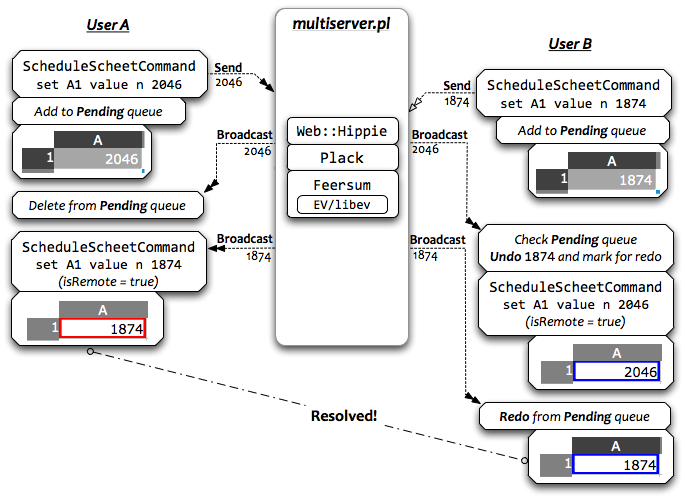
\includegraphics[width=1\textwidth]{resources/chapter-3-conflict-res.png}
    \caption{Mekanisme Penanganan Konflik \citep{EtherCalc}}
	\label{MekanismeKonflik}
\end{figure}

\section{Analisis Jenis \textit{Spreadsheet} yang Ditangani}
Pada Subbab \ref{JenisSpreadsheet} telah dijelaskan jenis-jenis \textit{spreadsheet} yang biasanya dibuat. Persentase jenis \textit{spreadsheet} terbesar yang dibuat berjenis \textit{data frame} dengan persentase 50.5\%. \textit{Data frame} merupakan tipe \textit{spreadsheet} yang terdiri dari 2 komponen utama: area nilai dan area atribut atau metadata (biasanya berada di atas dan atau di kiri area nilai). Karena tingginya angka penggunaan menggunakan tipe ini, aplikasi akan melakukan penanganan pada \textit{spreadsheet} bertipe \textit{data frame}.

Selain itu, persentase kedua ditempati oleh jenis \textit{spreadsheet} bertipe relasi yang memiliki persentase 22.0\%. Tipe relasi ini merupakan tipe \textit{spreadsheet} yang dapat langsung diubah ke model relasional. Biasanya berupa satu \textit{header} dan kumpulan baris data. Dengan tingginya persentase tipe ini serta miripnya tipe relasi dan \textit{data frame}, tipe ini juga dipilih untuk dapat ditangani oleh aplikasi.

Tipe lainnya yang teridentifikasi adalah tipe formulir, diagram, dan jadwal. Ketiga jenis ini memiliki penanganan yang berbeda-beda dan tidak memiliki sifat yang sama dengan tipe \textit{data frame} dan relasi. Sehingga, tipe ini tidak dijadikan fokus dalam pengembangan aplikasi untuk dapat ditangani. Dengan menangani hanya tipe \textit{data frame} dan relasi diharapkan telah dapat menangani 72.5\% kasus penggunaan \textit{spreadsheet} yang biasanya ditemui.

\section{Analisis Metode Interaksi Pengguna}
Di dalam pembangunan perangkat lunak \textit{spreadsheet} untuk mengurangi kesalahan, dapat diidentifikasikan dua metode interaksi yang dapat diimplementasi. Model interaksi yang pertama adalah menggunakan formulir sebagai basis masukan data dan metode yang kedua adalah menggunakan aplikasi \textit{spreadsheet} secara langsung sebagai media input data.
	\subsection{Berbasis Formulir}
	Metode interaksi ini menggunakan \textit{spreadsheet} sebagai tempat perancangan formulir. Pembuat formulir akan menentukan area label dan input secara manual serta diidentifikasikan berdasarkan warna atau properti lain yang unik pada sel tersebut. Formulir akan dibangkitkan oleh aplikasi agar menjadi bentuk HTML dan terhubung ke basis data. Pengisian data oleh pengguna dilakukan melalui formulir yang dibangkitkan dan dapat diakses melalui web. Beberapa cara dapat dilakukan untuk mengimplementasikan teknik ini antara lain, mengembangkan dari aplikasi \textit{spreadsheet} yang telah ada menggunakan \textit{plugin} atau membuat aplikasi baru yang dapat melakukan konversi otomatis menjadi formulir.

	\subsection{Berbasis \textit{Spreadsheet}}
	Metode interaksi berbasiskan \textit{spreadsheet} menggunakan antarmuka yang telah disediakan oleh aplikasi. Penggunaannya dilakukan dengan membuat format pengisian seperti membuat tabel pada \textit{spreadsheet} pada umumnya. Pada tabel harus terdapat label dan data sehingga metadata minimal yang dibutuhkan dapat dicapai. Fitur-fitur yang ada pada \textit{spreadsheet} juga tetap dapat digunakan saat pembuatan tabel yang diinginkan. Dari pembuatan tabel tersebut dilakukan identifikasi label dari data tersebut untuk selanjutnya diproses melalui penyaringan masukan dan dimasukan ke tabel yang sesuai yang ada di basis data. Untuk mengimplementasikan teknik ini harus mengubah kode pada program \textit{spreadsheet} atau mengekstensi fitur yang ada menggunakan \textit{plugin}. 

	\subsection{Perbandingan Metode Masukan}
	Kedua metode interaksi pengguna tersebut memiliki beberapa perbedaan dan efek terhadap penggunaannya baik bagi sistem maupun pengguna. Pada Tabel \ref{ModelInteraksi} dijabarkan perbandingan antara kedua metode interaksi pengguna tersebut.

	\begin{small}
	\begin{longtable}{ | p{3cm} | p{4cm} | p{4cm} | }
	    \caption{Perbandingan Metode Interaksi Pengguna}
	    \label{ModelInteraksi}\\ \hline
	    \centering\bfseries{Parameter} & \centering\bfseries{Berbasis Formulir} & \centering\bfseries{Berbasis \textit{Spreadsheet}} \tabularnewline \hline
	    \endfirsthead
	    \hline
	    \centering\bfseries{Parameter} & \centering\bfseries{Berbasis Formulir} & \centering\bfseries{Berbasis \textit{Spreadsheet}} \tabularnewline \hline
	    \endhead
	    Fungsionalitas & Berhasil memisahkan bagian operasional dan data. Pengguna hanya memodifikasi dan melakukan input pada bagian data. Bagian operasional hanya dapat dimodifikasi oleh pembuat formulir tersebut. & Jika tidak menggunakan proteksi terhadap sel yang dapat ditulis, tidak terjadi pemisahan antara data dan operasional sehingga beberapa kesalahan yang terjadi pada saat input masih dapat terjadi. \\ \hline
	    Teknologi & Dibutuhkan adanya algoritma tambahan untuk menangani formulir dan masukannya, serta melakukan konversi dan \textit{parsing} dari sel pada \textit{spreadsheet} ke dalam bentuk formulir. & Dibutuhkan algoritma dan logika \textit{parsing} yang lebih detil dan kompleks dalam menangani kasus-kasus table tertentu. \\ \hline
	    Antarmuka & Menggunakan antarmuka formulir yang kaku terurut dari atas ke bawah serta tidak dapat melihat hasil masukan secara langsung. & Struktur tabel atau masukan dapat disesuaikan dengan kebutuhan dan tidak perlu mempelajari hal lain jika sebelumnya telah menggunakan \textit{spreadsheet} sebagai media untuk memasukan data. \\ \hline
  	\end{longtable}
	\end{small}

  	Pada Tugas Akhir ini, akan dipilih metode masukan pengguna dengan berbasis \textit{spreadsheet} sehingga pengguna dapat dengan lebih mudah didalam menggunakannya karena tidak memerlukan pembelajaran kembali di dalam menggunakan aplikasi. Selain itu, data yang dimasukan lebih mudah untuk dilihat secara menyeluruh dibandingkan dengan berbasis formulir yang hanya dapat menerima satu masukan dalam suatu formulir.

\section{Analisis Penentuan Bagian Data dan Label}
Pada pembuatan \textit{spreadsheet} pada umumnya, didapatkan bahwa kebanyakan \textit{spreadsheet} pada umumnya berbentuk tabel yang terdiri dari dua unsur utama yakni data dan label atau disebut juga tipe \textit{data frame} \citep{Chen2013}. Bagian data merupakan bagian yang biasanya dinamis dan merupakan masukan pengguna. Bagian label merupakan bagian yang memberikan keterangan dan konteks mengenai data yang dimaksud. Pada Gambar \ref{DataFrameSederhana} dapat dilihat bahwa area dengan nomor 1 disebut sebagai label yang menjelaskan data-data dibawahnya yakni pada area nomor 2.

\begin{figure}[htb]
    \centering
    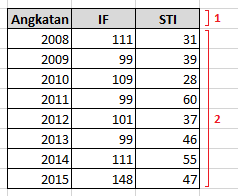
\includegraphics[width=0.3\textwidth]{resources/chapter-3-simple-dataframe.png}
    \caption{Contoh \textit{Data Frame} Sederhana}
	\label{DataFrameSederhana}
\end{figure}

	\subsection{Secara Manual}
	Penentuan label dan data dilakukan oleh pengguna secara langsung saat pembuatan tabel. Pengguna sendiri yang menentukan area mana yang merupakan label dan data mana yang dijelaskan oleh label tersebut. Dengan metode manual ini, pengguna dapat menyesuaikan bentuk tabel sesuai keinginan mereka. Metode ini menyerahkan sepenuhnya tanggungjawab keterhubungan sel label dan sel data kepada pengguna. Metode yang digunakan adalah menerima masukan dari pengguna berupa suatu \textit{script} yang mendefinisikan letak tabel, \textit{header}, dan data pada \textit{spreadsheet}.

	\subsection{Secara Otomatis}
	Penentuan secara otomatis dimulai dari pencarian tabel pada \textit{spreadsheet}. Hal ini dilakukan karena tabel dapat lebih dari satu pada sebuah \textit{spreadsheet}. Penentuan tabel dilakukan menggunakan algoritma k-Nearest Neighbour (kNN). Setelah tabel ditemukan, pencarian label dan data dapat menggunakan algoritma seperti yang telah dijelaskan pada Subbab \ref{metodepencarian}. Mekanisme untuk mengidentifikasi label dan data dapat dilakukan melalui 3 tahapan yakni, \textit{frame finder}, \textit{hierarchy extractor}, dan \textit{tuple builder}. Pada tahap pertama yakni \textit{frame finder} bertujuan untuk mengidentifikasi wilayah nilai (data) dan wilayah atribut (label) yang dapat berupa \textit{left attribute} maupun \textit{top attribute}. Tahap selanjutnya adalah \textit{hierarchy extractor} bertujuan untuk mendapatkan hirarki dari atribut-atribut yang ada sehingga label yang tertulis dapat dicari keterhubungan dan konteksnya terhadap data yang ada. Tahap terakhir adalah \textit{tuple builder} yang mentrasformasikan data dan label tersebut dalam bentuk \textit{tuple} yang dapat diterima oleh basis data relasional.

	\subsection{Perbandingan Metode Penentuan}
	Untuk mengetahui perbandingan kedua metode, pada Tabel \ref{MetodePenentuan} dijelaskan kelebihan dan kekurangan dua metode yang telah disebutkan sebelumnya.
	\begin{small}
	\begin{longtable}{ | p{3cm} | p{4cm} | p{4cm} | }
	    \caption{Perbandingan Metode Penentuan Data dan Label}
	    \label{MetodePenentuan}\\ \hline
	    \centering\bfseries{Keterangan} & \centering\bfseries{Manual oleh Pengguna} & \centering\bfseries{Otomatis} \tabularnewline \hline
	    \endfirsthead
	    \hline
	    \centering\bfseries{Keterangan} & \centering\bfseries{Manual oleh Pengguna} & \centering\bfseries{Otomatis} \tabularnewline \hline
	    \endhead
	    Kelebihan & Tingkat akurasi lebih tinggi karena data dan label yang ditentukan sesuai dengan keinginan pengguna. & Kenyamanan dalam penggunaan karena pengguna tidak perlu melakukan interferensi tambahan. Selain itu, sistem kemungkinan data dan label yang diambil dapat diubah ke dalam bentuk \textit{tuple} relasional lebih tinggi. \\ \hline
	    Kekurangan & Interferensi pengguna yang banyak dan mungkinnya data dan label tidak dapat dijadikan bentuk \textit{tuple} relasional. & Algoritma ini hanya optimal jika digunakan pada tabel yang terurut vertikal. \\ \hline
  	\end{longtable}
	\end{small}
  	Dari perbandingan diatas, dapat dilihat terdapat kekurangan dan kelebihan didalam menggunakan salah satu metode tersebut. Berdasarkan hal tersebut, yang akan dipilih sebagai metode penentuan data dan label adalah gabungan dari kedua metode tersebut. Sistem awalnya akan melakukan \textit{parsing} terhadap struktur yang telah dibuat oleh pengguna, kemudian pengguna dapat melihat hasil dari \textit{parsing} tersebut sehingga pengguna dapat memperbaiki jika terdapat hasil pelabelan yang salah. Dengan metode gabungan ini diharapkan dapat meningkatkan akurasi dan mengurangi kesalahan \textit{parsing} yang terjadi namun tetap memberikan kenyamanan terhadap pengguna serta menjaga agar hasil pelabelan tetap dapat diubah ke dalam bentuk \textit{tuple} relasional.

\section{Analisis Representasi Tabel pada \textit{Spreadsheet}}
Didalam pembuatan \textit{spreadsheet}, terdapat beberapa jenis tabel yang biasanya dibuat oleh pengguna dalam merepresentasikan data yang ingin disimpan. Pada jenis-jenis tabel tertentu, dibutuhkan transformasi bentuk tabel tersebut agar dapat dimasukkan ke dalam basis data bentuk relasional. Tipe-tipe tabel yang biasanya muncul di dalam pembuatan \textit{spreadsheet} beserta teknik transformasi yang akan digunakan adalah sebagai berikut:
\begin{enumerate}
	\item Tabel dengan \textit{header} berada di atas data
	\begin{figure}[htbp]
	    \centering
	    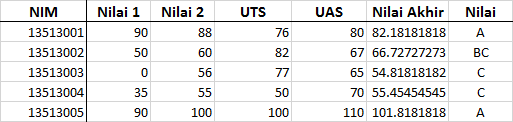
\includegraphics[width=0.8\textwidth]{resources/chapter-3-tabletype-1.png}
	    \caption{Tabel dengan \textit{Header} Berada Diatas Data}
		\label{TabelTipe1}
	\end{figure}\\
	Representasi tabel jenis ini dapat langsung dibuat ke dalam bentuk relasional tanpa harus mengubah struktur tabel. Contoh tabel jenis ini dapat dilihat pada Gambar \ref{TabelTipe1}. Bagian \textit{header} merupakan baris pertama pada tabel, dan baris kedua hingga seterusnya merupakan bagian data. Bentuk ini tidak membutuhkan transformasi agar dapat dimasukkan ke dalam basis data bentuk relasional.

	\item Tabel dengan \textit{header} berada di kiri dan atas data
	\begin{figure}[htbp]
	    \centering
	    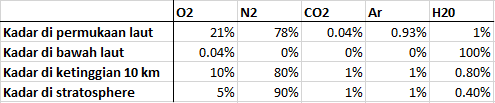
\includegraphics[width=0.8\textwidth]{resources/chapter-3-tabletype-2.png}
	    \caption{Tabel dengan \textit{Header} Berada di Kiri dan Atas Data}
		\label{TabelTipe2}
	\end{figure}\\
	Tabel dapat memiliki lebih dari satu \textit{header} di lokasi yang berbeda. Contoh tabel jenis ini dapat dilihat pada Gambar \ref{TabelTipe2}. Representasi tabel dimana \textit{header} bukan hanya di bagian atas saja, maka \textit{header} yang dianggap hanya yang di bagian atas. Bagian yang akan dianggap sebagai \textit{header} adalah kolom yang keseluruhannya berisi \textit{header} dan berada diatas data. Pada contoh diatas, \textit{header} adalah baris pertama. Sedangkan \textit{header} di kiri tabel yang satu baris dengan data akan dianggap data dengan nama \textit{header} yang dapat ditentukan oleh pengguna. Dengan demikian, representasi tabel tersebut akan menjadi mirip dengan tipe tabel sebelumnya. Representasi tabel setelah transformasi dapat dilihat pada Gambar \ref{TabelTipe2T}.\\
	\begin{figure}[htbp]
	    \centering
	    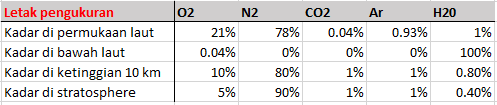
\includegraphics[width=0.8\textwidth]{resources/chapter-3-tabletype-2-transformed.png}
	    \caption{Transformasi Tabel dengan \textit{Header} Berada di Kiri dan Atas Data}
		\label{TabelTipe2T}
	\end{figure}

	\item Tabel dengan \textit{header} yang berhirarki
	\begin{figure}[htbp]
	    \centering
	    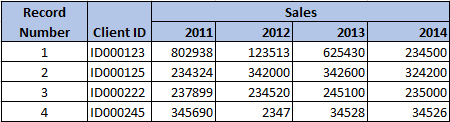
\includegraphics[width=0.7\textwidth]{resources/chapter-3-tabletype-3.png}
	    \caption{Tabel dengan \textit{Header} yang Berhirarki}
		\label{TabelTipe3}
	\end{figure}\\
	Tabel dapat memiliki \textit{header} yang berhubungan satu dengan yang lain dan membentuk hirarki seperti pada contoh Gambar \ref{TabelTipe3}. Tabel dengan \textit{header} yang memiliki hirarki akan tetap dianggap memiliki satu baris \textit{header}. Transformasi yang dilakukan adalah dengan menggabungkan kata-kata pada tiap \textit{header} dan dijadikan sebagai satu nama \textit{header}. Hasil transformasi tabel tersebut dapat dilihat pada Gambar \ref{TabelTipe3T}.\\
	\begin{figure}[htbp]
	    \centering
	    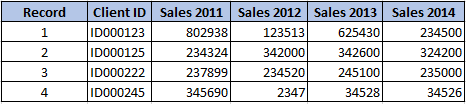
\includegraphics[width=0.75\textwidth]{resources/chapter-3-tabletype-3-transformed.png}
	    \caption{Transformasi Tabel dengan \textit{Header} yang Berhirarki}
		\label{TabelTipe3T}
	\end{figure}

	\item Tabel dengan data yang digabung
	\begin{figure}[htbp]
	    \centering
	    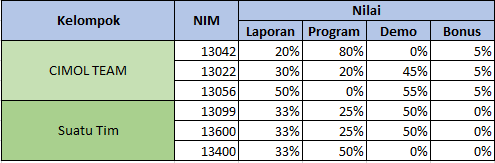
\includegraphics[width=0.8\textwidth]{resources/chapter-3-tabletype-4.png}
	    \caption{Tabel dengan Data yang Digabung}
		\label{TabelTipe4}
	\end{figure}\\
	Tabel dapat juga memiliki penggabungan sel pada bagian data seperti yang dapat dilihat pada contoh Gambar \ref{TabelTipe4}. Penggabungan sel ini biasanya digunakan sebagai penanda bahwa data pada setiap baris atau kolom yang digabung adalah sama. Sehingga, transformasi yang akan dilakukan adalah dengan memecah sel yang digabungkan tersebut dan mengisi setiap sel dengan konten yang sama dengan sel yang digabungkan. Hasil transformasi tabel dapat dilihat pada Gambar \ref{TabelTipe4T}.\\
	\begin{figure}[htbp]
	    \centering
	    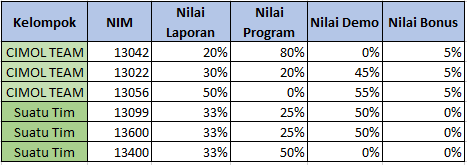
\includegraphics[width=0.75\textwidth]{resources/chapter-3-tabletype-4-transformed.png}
	    \caption{Transformasi Tabel dengan Data yang Digabung}
		\label{TabelTipe4T}
	\end{figure}
\end{enumerate}
Setelah ditransformasikan, tabel akan dapat dengan mudah dijadikan \textit{tuple} relasional sehingga dapat langsung dimasukkan ke dalam basis data relasional yang dipilih.

\section{Analisis Validasi Data}
Setelah pengguna memasukan datanya kedalam struktur yang telah ditetapkan, pengecekan data dilakukan. Tujuan dari mekanisme ini adalah untuk menghindari kesalahan masukan yang terjadi. Berdasarkan pada Subbab \ref{KesalahanPenggunaan}, terdapat dua jenis tipe kesalahan \citep{Panko1998} yang bisa terjadi pada penggunaan \textit{spreadsheet} yakni kesalahan kualitatif dan kesalahan kuantitatif. Dari kedua tipe tersebut, pada Tugas Akhir ini akan lebih ditekankan kepada kesalahan kuantitatif. Kesalahan kuantitatif diambil karena merupakan jenis kesalahan yang dapat ditangani oleh aplikasi, sedangkan jenis kesalahan kuantitatif lebih berkaitan pada aturan dan konvensi pembuatan \textit{spreadsheet}.

Berdasarkan penelitian yang telah disebutkan pada Subbab \ref{KesalahanPenggunaan}, diketahui bahwa pengurangan kesalahan \textit{formula} sangat dipengaruhi oleh faktor umur, indeks prestasi, dan pengalaman pemrograman yang dapat dicapai oleh seseorang jika berlatih dan terbiasa. Namun, jenis kesalahan lain tidak dipengaruhi oleh faktor-faktor ini, sehingga tingkat kesalahan yang terjadi cukuplah konsisten tidak tergantung pengalaman. Sehingga, jenis kesalahan yang akan ditangani oleh aplikasi ini akan lebih difokuskan pada kesalahan-kesalahan yang sulit dihilangkan bahkan jika pengguna telah berpengalaman.

Jenis kesalahan yang akan ditangani adalah kesalahan \textit{clerical} dan non-material, \textit{rule violations}, dan kesalahan \textit{data-entry}. Dari kesalahan-kesalahan tersebut, maka terdapat tiga hal utama yang divalidasi pada aplikasi ini, yakni:
\begin{enumerate}
	\item Validasi tipe data. Contohnya, data masukan yang seharusnya berupa \textit{integer} tidak dapat menerima masukan berupa \textit{string}.
	\item Validasi domain masukan. Pengguna dapat juga mengatur rentang \textit{integer} yang boleh dijadikan masukan atau \textit{string} apa saja yang dapat diterima oleh sistem.
	\item Validasi relasi data. Data masukan dapat berupa nilai yang harus ada pada tabel lain, contohnya terdapat 2 tabel yakni nilai mahasiswa dan identitas mahasiswa. Tabel nilai mahasiswa memiliki kolom NIM yang nilainya harus ada pada tabel identitas mahasiswa. Pada \textit{spreadsheet} biasanya hal ini diatasi dengan menggunakan perintah VLOOKUP.
\end{enumerate}

Kesalahan \textit{clerical} dan non-material diharapkan dapat ditangani menggunakan validasi tipe data dan domain masukan. Kesalahan \textit{data-entry} dan \textit{rule violations} diharapkan dapat ditangani menggunkan validasi tipe data, validasi domain, dan validasi relasi data.

Sistem akan melakukan validasi terhadap ketiga hal tersebut dan menolak data masukan sehingga pengguna dapat memperbaiki data. Validasi akan dilakukan pada saat data akan dimasukkan ke dalam basis data. Alur validasi ini dapat dilihat pada Subbab \ref{Aluralur}.

\section{Analisis Penyimpanan Data}
Terdapat tiga permasalahan pada penyimpanan data yang perlu dianalisis yakni; jenis penyimpanan data yang digunakan, alur pengguna melakukan penyimpanan data tersebut, dan perubahan pada data di basis data. Kedua masalah ini akan dijelaskan pada dua subbab berikut.

	\subsection{Jenis Penyimpanan Data} \label{JenisPenyimpanan}
	Data yang telah dimasukan oleh pengguna baik data bentuk struktur \textit{spreadsheet} maupun data masukan pada struktur disimpan ke dalam basis data yang presisten. Terdapat 2 jenis data yang harus disimpan ke dalam basis data di dalam membangun aplikasi \textit{spreadsheet} ini, yakni:

	\begin{enumerate}
		\item Penyimpanan \textit{File Spreadsheet} \\
		\textit{File spreadsheet} yang dimaksud adalah data struktural seperti \textit{value} pada suatu sel, \textit{properties} suatu sel seperti warna, \textit{border}, dan \textit{alignment}, serta hal-hal lain yang berhubungan dengan bagaimana suatu \textit{file spreadsheet} ditampilkan pada aplikasi. Tipe penyimpanan yang dapat digunakan untuk menampung data ini adalah NoSQL karena tipe ini cocok untuk menangani data yang kurang terstruktur seperti \textit{file spreadsheet} yang struktur penempatan datanya berbeda tiap pengguna. Cara penyimpanan yang cocok untuk menangani struktur ini adalah \textit{document based} atau \textit{key-value}. Sehingga proses penyimpanan \textit{file spreadsheet} akan menggunakan mekanisme yang sudah disediakan oleh aplikasi EtherCalc dengan menggunakan redis.

		\item Penyimpanan Data dan Label \\
		Data yang disimpan merupakan hasil dari pendeteksian label dan data yang akan diubah menjadi \textit{tuple} relasional yang dapat diterima oleh basis data relasional. Contoh pengubahan yang terjadi dapat dilihat pada Gambar \ref{RelationalTuple}.

		\begin{figure}[htb]
		    \centering
		    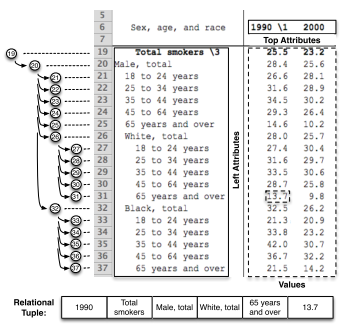
\includegraphics[width=0.6\textwidth]{resources/chapter-3-relational-tuple.png}
		    \caption{Contoh \textit{Tuple} Relasional}
			\label{RelationalTuple}
		\end{figure}

		Setelah data dan label dijadikan \textit{tuple} relasional, \textit{tuple} dimasukan ke dalam basis data dengan menggunakan operasi \textit{insert} ke dalam tabel pada basis data. Tipe penyimpanan yang cocok digunakan adalah basis data relasional (SQL) karena data yang dibuat dalam bentuk tabel pada umumnya dapat dikonversikan menjadi \textit{tuple} relasional.
	\end{enumerate}

	\subsection{Alur Penyimpanan Data}
	Dengan adanya dua jenis penyimpanan yang digunakan seperti telah dijelaskan pada Subbab \ref{JenisPenyimpanan} terdapat dua kemungkinan alur penyimpanan data, yakni:
	\begin{enumerate}
		\item Penyimpanan ke basis data dilakukan setiap mendapatkan masukan pengguna
		\item Penyimpanan ke basis data menunggu perintah dari pengguna
	\end{enumerate}
	Jika menggunakan alur penyimpanan basis data yang dilakukan setiap mendapatkan masukan, terdapat beberapa kelebihan yakni sinkronisasi antara basis data yang menyimpan \textit{file spreadsheet} yakni redis dan basis data yang menyimpan data yakni basis data relasional yang dipilih. Kedua basis data ini akan memiliki data yang sama setiap waktu. Namun kelemahan alur ini adalah performansi yang akan menurun diakibatkan sistem pendeteksian label dan data yang harus dilakukan setiap saat menerima masukan. Kelemahan lainnya adalah akan sulit untuk mengembangkan aplikasi menggunakan \textit{user access control} karena sulit menentukan kapan dan oleh siapa data boleh dimasukkan ke dalam basis data.

	Menggunakan alur penyimpanan yang menunggu perintah dari pengguna, memiliki kelebihan performansi yang lebih baik dibandingkan alur sebelumnya karena penyimpanan dilakukan \textit{on demand}. Selain itu, jika akan mengembangkan aplikasi dengan \textit{user access control} akan lebih mudah untuk menentukan siapa yang memiliki akses untuk melakukan penyimpanan. Kelemahan dari alur ini adalah tidak sinkronnya kedua basis data.

	Dari pertimbangan tersebut, alur yang akan digunakan pada aplikasi ini adalah penyimpanan ke basis data yang menunggu perintah dari pengguna karena kelebihannya pada sisi performa dan \textit{user access control}. Selain itu, tidak sinkronnya antara kedua basis data bukan merupakan masalah karena data yang ingin dikumpulkan merupakan data akhir dan data tiap perubahan yang dilakukan tidak begitu dipedulikan.

	\subsection{Perubahan pada Data di Basis Data}
	Kasus yang dapat terjadi pada basis data tempat penyimpanan data yang berasal dari \textit{spreadsheet} adalah diubahnya data tersebut secara manual oleh entitas lain. Pada aplikasi yang dibuat, aplikasi hanya bekerja sebagai media untuk mengumpulkan data sehingga perubahan yang terjadi pada basis data, tidak akan ditampilkan kembali menjadi bentuk \textit{spreadsheet} pada aplikasi. Selain itu, perubahan data langsung pada basis data tanpa melalui media yang disediakan sangat tidak disarankan.

\section{Analisis Interaksi antar \textit{Spreadsheet}}
Data yang dikumpulkan pada dua atau lebih \textit{spreadsheet} dapat diklasifikasikan menjadi empat tipe berdasarkan fragmen data yang dikumpulkan yakni; tidak berhubungan, horizontal, vertikal, dan gabungan.
	\subsection{Fragmen Tidak Berhubungan}
	Dua atau lebih \textit{spreadsheet} dapat dikatakan tidak saling berpotongan fragmennya jika \textit{spreadsheet} tersebut tidak menyimpan data pada tabel yang sama pada basis data. Pada kasus tersebut, data pada kedua atau lebih \textit{spreadsheet} dapat dianggap tidak saling melengkapi dan dapat berdiri sendiri.
	
	\subsection{Fragmen Horizontal}
	Fragmen horizontal terjadi ketika dua atau lebih \textit{spreadsheet} menyimpan pada tabel basis data yang sama dimana data yang disimpan memiliki jumlah, nama, dan konteks kolom yang sama. Pada kasus tersebut, data pada dua atau lebih \textit{spreadsheet} akan digabungkan pada satu tabel yang sama secara horizontal. Contoh gambaran pengabungan data dapat dilihat pada Gambar \ref{HorizontalMerge}.

	\begin{figure}[htb]
	    \centering
	    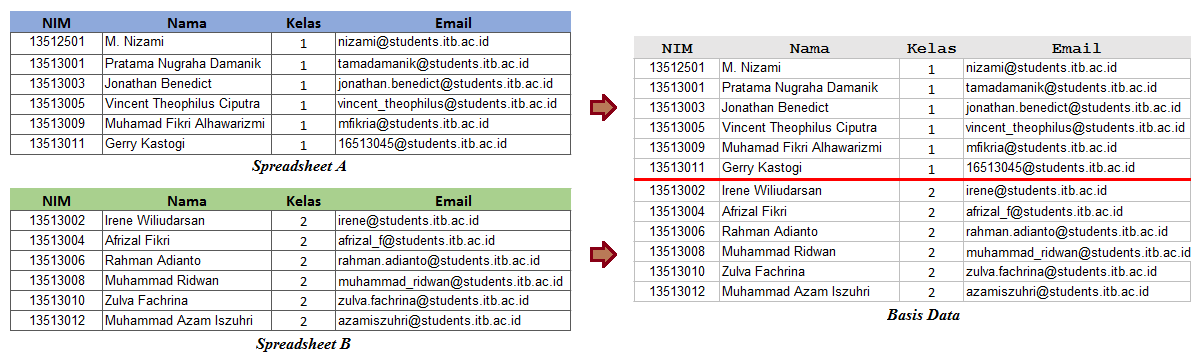
\includegraphics[width=1\textwidth]{resources/chapter-3-horizontal-merge.png}
	    \caption{Contoh Penggabungan Horizontal}
		\label{HorizontalMerge}
	\end{figure}

	Pada gambar, data pada \textit{spreadsheet} A dan \textit{spreadsheet} B digabungkan pada satu tabel pada basis data secara horizontal (diilustrasikan dengan garis merah). Pada kasus tersebut, NIM tidak didefinisikan sebagai nilai yang unik, sehingga jika terdapat NIM yang sama pada lebih dari satu \textit{spreadsheet} maka data akan tetap digabungkan secara horizontal pada data yang sudah ada bukan menulis kembali nilai pada NIM yang bersesuaian. Namun, jika nilai NIM didefinisikan sebagai unik, maka jika NIM terdapat di lebih dari satu \textit{spreadsheet} akan ditimpa dan ditulis kembali nilainya pada NIM yang sesuai.

	\subsection{Fragmen Vertikal}
	Fragmen vertikal terjadi ketika dua atau lebih \textit{spreadsheet} menyimpan pada tabel basis data yang sama dimana data yang disimpan memiliki satu kolom unik dengan nama dan konteks yang sama dan kolom lainnya dapat berbeda dari segi jumlah , nama, dan konteks di masing-masing \textit{spreadsheet}. Pada kasus ini, data pada dua atau lebih \textit{spreadsheet} akan digabungkan pada satu tabel yang sama secara vertikal. Contoh gambaran pengabungan data dapat dilihat pada Gambar \ref{VerticalMerge}.

	\begin{figure}[htb]
	    \centering
	    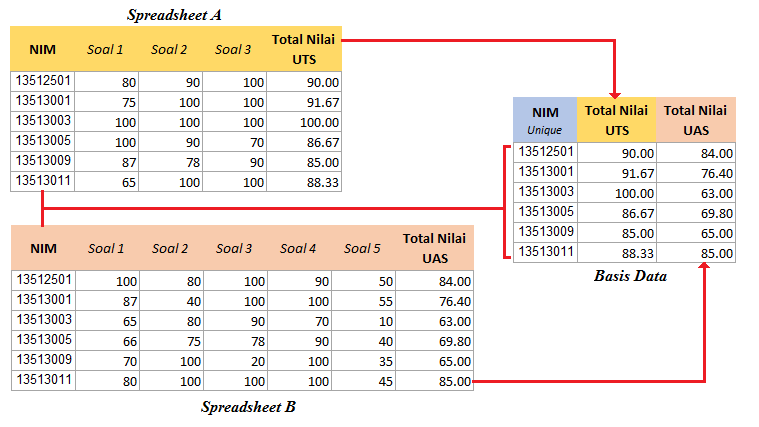
\includegraphics[width=0.9\textwidth]{resources/chapter-3-vertical-merge.png}
	    \caption{Contoh Penggabungan Vertikal}
		\label{VerticalMerge}
	\end{figure}

	Penggabungan secara vertikal membutuhkan suatu kolom \textit{key} dan unik yang dapat dijadikan patokan penggabungan data pada suatu baris data. Untuk masing-masing \textit{spreadsheet} yang akan digabungkan datanya, harus memiliki kolom \textit{key} dan unik yang sama dengan konteks data yang sama. Pada contoh pada gambar, kolom unik yang dipilih adalah kolom NIM. Penggabungan data dilakukan dengan mengambil data dari \textit{spreadsheet} A yakni data nilai UTS, dan dari \textit{spreadsheet} B yakni data nilai UAS, lalu dimasukkan ke dalam basis data pada tabel yang dipilih.

	\subsection{Fragmen Horizontal dan Vertikal}
	Fragmen gabungan ini terjadi ketika data yang digabungkan ada yang memiliki perbedaan kolom, ada juga yang tidak, atau juga dapat merupakan gabungan semua kolom yang ada. Contoh kasus yang dapat terjadi dapat dilihat pada Gambar \ref{BothTableMerge}.

	\begin{figure}[htb]
	    \centering
	    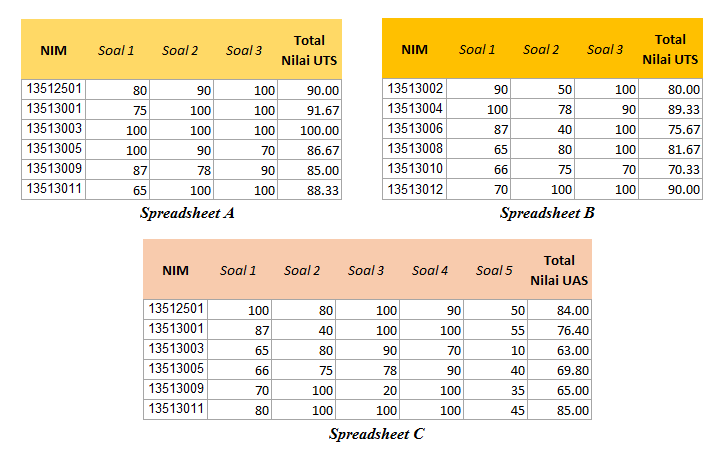
\includegraphics[width=0.9\textwidth]{resources/chapter-3-both-merge.png}
	    \caption{Contoh Tabel Penggabungan}
		\label{BothTableMerge}
	\end{figure}

	Terdapat tiga \textit{spreadsheet} dimana data pada \textit{spreadsheet} A dan \textit{spreadsheet} C memiliki jumlah kolom yang sama dan dapat digabung secara horizontal. Sedangkan, \textit{spreadsheet} A dan \textit{spreadsheet} B memiliki jumlah kolom yang berbeda namun kolom unik yang sama yakni NIM sehingga dapat digabungkan secara vertikal. Hasil penggabungan ketiga \textit{spreadsheet} ini akan menjadi tabel yang dapat dilihat pada Gambar \ref{BothMerge}.

	\begin{figure}[htb]
	    \centering
	    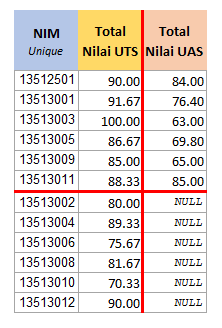
\includegraphics[width=0.3\textwidth]{resources/chapter-3-both-merge-db.png}
	    \caption{Contoh Penggabungan Horizontal dan Vertikal}
		\label{BothMerge}
	\end{figure}

	Karena dari hasil penggabungan data tidak semua kolom dapat dipenuhi, maka terdapat kolom yang berisikan NULL sebagai penanda bahwa kolom tersebut kosong dan tidak mendapatkan data dari \textit{spreadsheet}.


\section{Analisis Alur Kerja dan Alur Aplikasi} \label{Aluralur}
Pada subbab ini, akan dijelaskan perbedaan alur kerja manusia dalam pengumpulan data menggunakan aplikasi yang dibuat dengan aplikasi biasa. Selain itu, akan dijelaskan juga perubahan alur aplikasi di dalam menangani masukan pengguna.

\subsection{Alur Kerja}
Terdapat perbedaan alur kerja yang terjadi jika pengguna menggunakan aplikasi yang dibuat pada Tugas Akhir. Alur kerja lama dapat dilihat pada Gambar \ref{GambarWorkflowKerjaBiasa} dan alur kerja pada aplikasi \textit{spreadsheet} yang dibagun dapat dilihat pada Gambar \ref{GambarWorkflowKerja}.

\begin{figure}[htb]
    \centering
    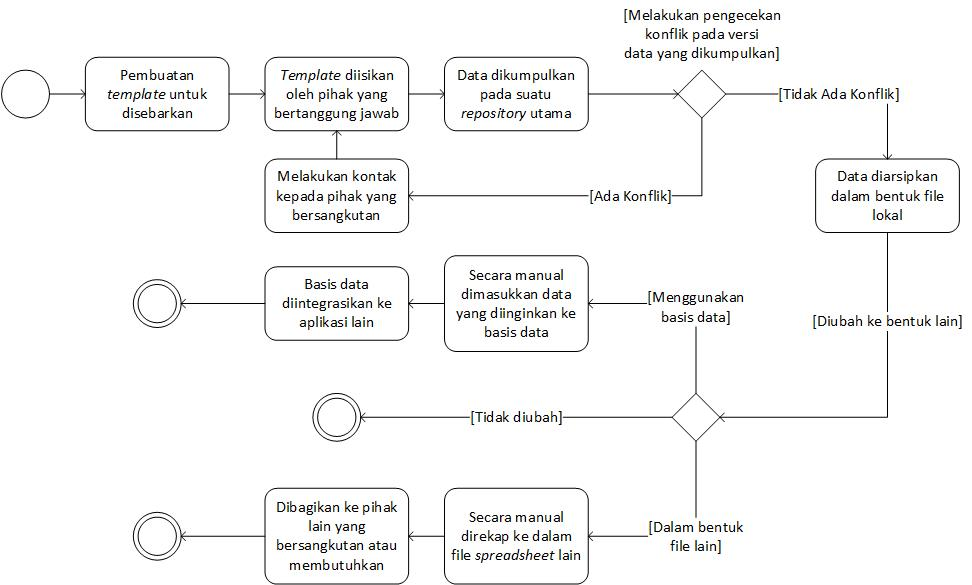
\includegraphics[width=0.7\textwidth]{resources/chapter-3-workflow-kerja-biasa.jpg}
    \caption{Alur Aplikasi \textit{Spreadsheet} Biasa}
	\label{GambarWorkflowKerjaBiasa}
\end{figure}

\begin{figure}[htb]
    \centering
    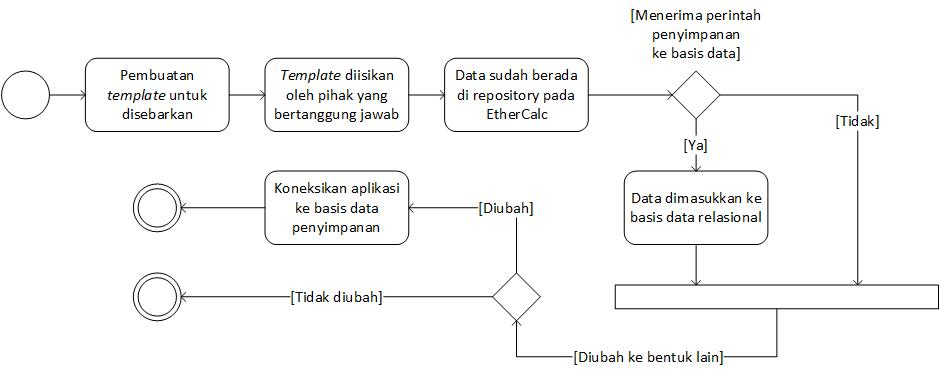
\includegraphics[width=1\textwidth]{resources/chapter-3-workflow-kerja.jpg}
    \caption{Alur Aplikasi \textit{Spreadsheet} yang Akan Dibuat}
	\label{GambarWorkflowKerja}
\end{figure}

Seperti yang digambarkan pada alur tersebut, dengan menggunakan aplikasi yang dikembangkan akan mengurangi alur yang dibutuhkan untuk mengumpulkan data. Pengurangan alur terjadi pada bagian penanganan konflik pada versi-versi \textit{spreadsheet} yang berbeda dan menjadi hanya dibutuhkan satu cara untuk mengubah data ke bentuk lain, yakni menggunakan koneksi basis data.

\subsection{Alur Aplikasi}
Aplikasi yang dibuat akan mengubah alur penggunaan \textit{spreadsheet} yang umum dengan menambahkan mekanisme-mekanisme yang dibutuhkan. Alur aplikasi yang lama dapat dilihat pada Gambar \ref{GambarWorkflowBiasa} dan aplikasi \textit{spreadsheet} yang dibangun pada Tugas Akhir ini pada Gambar \ref{GambarWorkflow}.

\begin{figure}[htb]
    \centering
    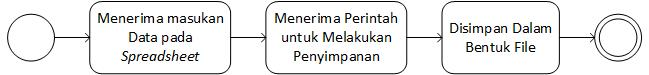
\includegraphics[width=0.7\textwidth]{resources/chapter-3-workflow-biasa.jpg}
    \caption{Alur Aplikasi \textit{Spreadsheet} Biasa}
	\label{GambarWorkflowBiasa}
\end{figure}

\begin{figure}[htb]
    \centering
    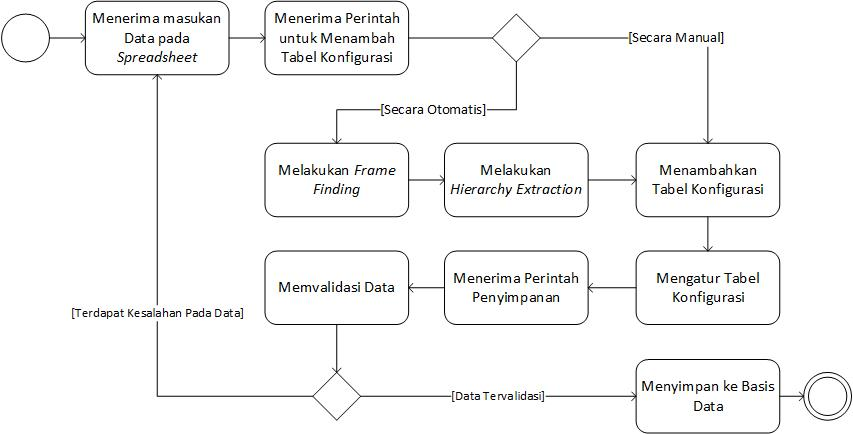
\includegraphics[width=1\textwidth]{resources/chapter-3-workflow.jpg}
    \caption{Alur Aplikasi \textit{Spreadsheet} yang Akan Dibuat}
	\label{GambarWorkflow}
\end{figure}

Dapat dilihat bahwa terdapat proses tambahan yang dilakukan pada aplikasi yang akan dibuat. Proses tersebut terdiri dari pencarian bagian label dan data jika menggunakan pencarian otomatis, pengaturan tabel konfigurasi untuk aturan masukkan ke basis data, serta proses validasi. Fokus aplikasi ini hanya sampai menyimpan data pada basis data, sehingga permasalahan \textit{input} dan \textit{output} berupa \textit{file} tidak ditangani. Alur kolaborasi bukan merupakan fokus pengembangan Tugas Akhir ini sehingga akan ditangani oleh aplikasi \textit{spreadsheet} yang dipilih.

% \section{Rencana Tindak Lanjut}
% Berdasarkan analisa yang telah dijelaskan pada bab-bab sebelumnya, pada Tugas Akhir ini akan dibangun aplikasi \textit{spreadsheet} dengan menggunakan EtherCalc sebagai teknologi utama. Pada Subbab \ref{TeknologiSpreadsheet} telah dijelaskan bahwa EtherCalc merupakan perangkat lunak \textit{spreadsheet} yang \textit{open source} dan memiliki kemampuan kolaborasi didalam penggunaannya. Sehingga dengan menggunakan EtherCalc, aspek-aspek yang telah dijelaskan pada Subbab \ref{AspekAplikasi} yang harus ada didalam pembangunan \textit{spreadsheet} ini sudah dapat dipenuhi. Pada Tugas Akhir ini akan dilakukan pengembangan dari EtherCalc yang berupa identifikasi label dan data, penanganan validasi data dan keterhubungannya dengan basis data relasional. Alur kerja dari aplikasi \textit{spreadsheet} yang akan dibuat dapat dilihat pada Gambar \ref{GambarWorkflow} pada Subbab \ref{AspekAplikasi}.